\newcommand{\newAlgorithm}[1]{
	%\newpage
	\section{#1}
	%\nopagebreak[4]
	\lstinputlisting{#1}
}

\begin{document}

%\renewcommand{\baselinestretch}{0.25}\normalsize
\setlength{\cftbeforesecskip}{3.3pt}
\tableofcontents
%\renewcommand{\baselinestretch}{1.0}\normalsize

%\newpage
\newAlgorithm{final/template/template.cpp}

\section{Practice round}
\begin{itemize}
\item Посабмитить задачи каждому человеку.
\item Распечатать решение.
\item IDE для джавы.
\item Сравнить скорость локального компьютера и сервера.
\item Проверить \texttt{int128}.
\item Проверить прагмы. Например, на \texttt{bitset}.
\end{itemize}

\newAlgorithm{final/stuff/debug.cpp}
	
\newAlgorithm{final/template/fastIO.cpp}
\newAlgorithm{final/template/optimizations.cpp}
\newAlgorithm{final/template/useful.cpp}
\newAlgorithm{final/template/Template.java}
\newAlgorithm{final/template/bitset.cpp}
\newAlgorithm{final/template/treapNoRec.cpp}

\newpage
\newAlgorithm{final/numeric/fft.cpp}
\newAlgorithm{final/numeric/fst.cpp}
\newAlgorithm{final/numeric/fftint.cpp}
\newAlgorithm{final/numeric/berlekamp.cpp}
\newAlgorithm{final/numeric/blackbox.cpp}
\newAlgorithm{final/numeric/crt.cpp}
\newAlgorithm{final/numeric/extendedgcd.cpp}
\newAlgorithm{final/numeric/mulMod.cpp}
\newAlgorithm{final/numeric/modReverse.cpp}
\newAlgorithm{final/numeric/pollard.cpp}
\newAlgorithm{final/numeric/poly.cpp}
\newAlgorithm{final/numeric/simplex.cpp}
\newAlgorithm{final/numeric/sumLine.cpp}
\newAlgorithm{final/numeric/integrate.cpp}
\newAlgorithm{final/numeric/rootsPolynom.cpp}
\newAlgorithm{final/numeric/phiFunction.cpp}
\newAlgorithm{final/numeric/partition.cpp}

%\newpage
\newAlgorithm{final/geom/commonTangents.cpp}
\newAlgorithm{final/geom/halfplaneIntersection.cpp}
\newAlgorithm{final/geom/minDisc.cpp}
\newAlgorithm{final/geom/convexHull3D-N2.cpp}
\newAlgorithm{final/geom/convexDynamic.cpp}
\newAlgorithm{final/geom/polygonArcCut.cpp}
\newAlgorithm{final/geom/polygonTangent.cpp}
\newAlgorithm{final/geom/checkPlaneInt.cpp}
\newAlgorithm{final/geom/furthestPoints.cpp}
\newAlgorithm{final/geom/chtDynamic.cpp}
\newAlgorithm{final/geom/rotate3D.cpp}
\newAlgorithm{final/geom/circleInter.cpp}
\newAlgorithm{final/geom/sphericalDistance.cpp}
\newAlgorithm{final/geom/delaunayN4.cpp}

%\newpage
\newAlgorithm{final/strings/eertree.cpp}
\newAlgorithm{final/strings/manacher.cpp}
\newAlgorithm{final/strings/sufAutomaton.cpp}
\newAlgorithm{final/strings/sufTree.cpp}
\newAlgorithm{final/strings/sufArray.cpp}
\newAlgorithm{final/strings/sufArrayLinear.cpp}
\newAlgorithm{final/strings/duval.cpp}

\newpage
\newAlgorithm{final/graphs/alphaBetta.cpp}
\newAlgorithm{final/graphs/dominatorTree.cpp}
\newAlgorithm{final/graphs/generalMatching.cpp}
\newAlgorithm{final/graphs/heavyLight.cpp}
\newAlgorithm{final/graphs/hungary.cpp}
\newAlgorithm{final/graphs/minCost.cpp}
\newAlgorithm{final/graphs/minCostNegCycle.cpp}
\newAlgorithm{final/graphs/retro.cpp}
\newAlgorithm{final/graphs/mincut.cpp}
%\newAlgorithm{final/graphs/twoChinese.cpp}
\newAlgorithm{final/graphs/twoChineseFast.cpp}
\newAlgorithm{final/graphs/linkcut.cpp}
\newAlgorithm{final/graphs/chordaltree.cpp}
\newAlgorithm{final/graphs/minimization.cpp}
\newAlgorithm{final/graphs/matroidIntersection.cpp}
\newAlgorithm{final/graphs/compressTree.cpp}

%\newpage
Про диаграмму Вороного: Если соединить все сайты, соответствующие смежным ячейкам диаграммы Вороного, получится триангуляция Делоне для этого множества точек.
Наивно: Будем пересекать полуплоскости по свойству ячейки диаграммы. $\mathcal{O}(n^2 \log n)$

\texttt{dbl Simpson() \{ return (F(-1) + 4 * F(0) + F(1)) / 6; \}}

\texttt{dbl Runge2() \{ return (F(-sqrtl(1.0 / 3)) + F(sqrtl(1.0 / 3))) / 2; \}}

\texttt{dbl Runge3() \{ return (F(-sqrtl(3.0 / 5)) * 5 + F(0) * 8 + F(sqrtl(3.0 / 5)) * 5) / 18; \}}
Simpson и Runge2 -- точны для полиномов степени $\le 3$
Runge3 -- точен для полиномов степени $\le 5$

---

Явный Рунге-Кутт четвертого порядка, ошибка $\mathcal{O}(h^4)$

$y' = f(x, y)$

$x_{n + 1} = x_n + h, y_{n+1} = y_n + (k1 + 2 \cdot k2 + 2 \cdot k3 + k4) \cdot h / 6$

$k1 = f(xn, yn)$

$k2 = f(xn + h/2, yn + h/2 \cdot k1)$

$k3 = f(xn + h/2, yn + h/2 \cdot k2)$

$k4 = f(xn + h, yn + h \cdot k3)$

---

if $a^{(p-1)/f} \ne 1 (mod p)$ for all factors $f$ of $p-1$, $a$ is a primitive root modulo $p$.
Now, we want $w^n=1 (mod p)$ (here $n$ is our transform length). 
So we find a prime of the form $p=kn+1$.
$w=r^k (mod p)$
That's it. Now $w^n=r^{kn}=r^{p-1}=1 (mod p)$. And $w^n=1$ but $w^m != 1$ if $m < n$. So it works.

---

Извлечение корня по простому модулю (от Сережи)
$3 \leq p$, $1 \leq a < p$, найти $x^2 = a$
\begin{enumerate}
\item Если $a^{\frac{p - 1}{2}} \ne 1$, return $-1$
\item Выбрать случайный $1 \leq i < p$
\item $T(x) = (x + i)^{(p - 1)/2} mod (x^2 - a) = bx + c$
\item Если $b \ne 0$ то вернуть $\frac{c}{b}$, иначе к шагу 2)
\end{enumerate}

---

Чтобы посчитать количество остовных деревьев в неориентированном графе $G$:

    создать матрицу $N \times N$ \texttt{mat}, для каждого ребра ($a, b$):
    
	\texttt{mat[a][a]++, mat[b][b]++, mat[a][b]--, mat[b][a]--}.
	
	Удалить последнюю строку и столбец, взять дискриминант.
	
---

Лемма Бернсайда:

Группа $G$ действует на множество $X$
Тогда число классов эквивалентности = $\frac{\sum_{g \in G} {|f(g)|}}{|G|}$,
где $f(g)$ = число $x$ (из $X$) : $g(x) == x$

---

Число простых быстрее $\mathcal{O}(n)$: 

$dp(n, k)$ -- число чисел от $1$ до $n$ в которых все простые $\ge p[k]$
$dp(n, 1) = n$, $dp(n, j) = dp(n, j + 1) + dp(n / p[j], j)$, $\Rightarrow$ $dp(n, j + 1) = dp(n, j) - dp(n / p[j], j)$

Если $p[j]$, $p[k] > \sqrt{n}$, то $dp(n, j) + j == dp(n, k) + k$

Делаешь все оптимайзы сверху, но не считаешь глубже dp(n, k), n < K
Потом фенвиком+сортировкой подсчитываешь за (K+Q)log все эти запросы
Делаешь во второй раз, но на этот раз берешь прекальканные значения

Если $\sqrt{n} < p[k] < n$, то (число простых до $n$) $= dp(n, k) + k - 1$

---

$sum(k=1..n) k^2 = n(n+1)(2n+1)/6$

$sum(k=1..n) k^3 = n^2(n+1)^2/4$


Чиселки: 

Фибоначчи
45:  1134903170
46:  1836311903
47:  2971215073
91:  4660046610375530309
92:  7540113804746346429
93:  12200160415121876738

Числа с кучей делителей
20: d(12)=6
50: d(48)=10
100: d(60)=12
1000: d(840)=32
$10^4$: d(9240)=64
$10^5$: d(83160)=128
$10^6$: d(720720)=240
$10^7$: d(8648640)=448
$10^8$: d(91891800)=768
$10^9$: d(931170240)=1344
$10^{11}$: d(97772875200)=4032
$10^{12}$: d(963761198400)=6720
$10^{15}$: d(866421317361600)=26880
$10^{18}$: d(897612484786617600)=103680

Bell numbers:
$B(p^m + n) = mB(n) + B(n + 1) (mod p)$

0:1, 1:1, 2:2, 3:5, 4:15, 5:52, 6:203, 7:877, 8:4140, 9:21147,
10:115975, 11:678570, 12:4213597, 13:27644437, 14:190899322,
15:1382958545, 16:10480142147, 17:82864869804, 18:682076806159,
19:5832742205057, 20:51724158235372, 21:474869816156751,
22:4506715738447323, 23:44152005855084346

Catalan numbers:
$C_n = \binom{2n}{n} / (n + 1) = \binom{2n + 1}{n} / (2n + 1) = \binom{2n}{n} - \binom{2n}{n - 1}$

0:1, 1:1, 2:2, 3:5, 4:14, 5:42, 6:132, 7:429, 8:1430, 9:4862,
10:16796, 11:58786, 12:208012, 13:742900, 14:2674440,
15:9694845, 16:35357670, 17:129644790, 18:477638700,
19:1767263190, 20:6564120420, 21:24466267020, 22:91482563640,
23:343059613650, 24:1289904147324, 25:4861946401452

Partitions numbers:
see partition.cpp

0:1, 1:1, 2:2, 3:3, 4:5, 5:7, 6:11, 7:15, 8:22, 9:30, 10:42, 20:627, 30:5604, 40:37338, 50:204226, 60:966467, 70:4087968, 80:15796476, 90:56634173, 100:190569292

Stirling numbers of the second kind

$S(n, k) = S(n - 1, k - 1) + kS(n - 1, k)$
$S(n, 1) = S(n, n) = 1$
$S(n, k) = \frac{1}{k!} \sum_{j=0}^{k}{(-1)^{k - j}\binom{k}{j}j^n}$

$$prod (k=1..+inf) (1-x^k) = \sum_{q=-inf}^{+inf} {(-1)^q x^{(3q^2-q)/2}}$$

$$\sum_{k = 0}^{n}{k \binom{n}{k}} = n 2^{n - 1}$$

$$\sum_{j = 0}^{k}{\binom{m}{j} \binom{n - m}{k - j}} = \binom{n}{k}$$

$$\sum_{j = 0}^{m}{\binom{m}{j}^2} = \binom{2m}{m}$$

$$\sum_{m = 0}^{n}{\binom{m}{j}\binom{n - m}{k - j}} = \binom{n + 1}{k + 1}$$

$$\sum_{m = k}^{n}{\binom{m}{k}} = \binom{n + 1}{k + 1}$$

$$\sum_{k = 0}^{\lfloor n / 2 \rfloor}{\binom{n - k}{k}} = F(n + 1)$$

$$\sum_{j = 0}^{k}{(-1)^{j} \binom{n}{j}} = (-1)^k \binom{n - 1}{k}$$

$$\sum_{k = q}^{n}{\binom{n}{k} \binom{k}{q}} = 2^{n - q}\binom{n}{q}$$

$$\sum_{k =-a}^{a}{(-1)^k \binom{a + b}{a + k} \binom{b + c}{b + k} \binom{c + a}{c + k} } = \frac{(a + b + c)!}{a! b! c!}$$

Формулы:

$F(n, r) = rn^{n - 1 - r}$~--- число лесов, у которых $n$ вершин, $r$ компонент и каждая компонента
содержит свою вершину $i \in 1, 2, \dots , r$. 

$U_n = \sum_{k=3}^{n}{\binom{n}{r} \frac{(r - 1)!}{2} \cdot F(n, r)}$~--- число уницикликов

$M_n = M_{n - 1} + \sum_{i=0}^{n-2}{M_i M_{n - 2 - i}} = \frac{2n + 1}{n + 2}M_{n - 1} + \frac{3n - 3}{n + 2}M_{n - 2}$~--- 
количество способов провести непересекающиеся диагонали среди $n$ точек на круге.

$nD(n) = 3(2n - 1)D(n - 1) - (n - 1)D(n - 2)$

$D(m, n) = \sum_{k=0}^{\min(m, n)}{\binom{m}{k} \binom{n}{k} 2^k}$~--- количество путей черепашки с возможностью ходить по диагонали.

$C(l, r) = \binom{n}{n / 2 - r / 2} - \binom{n}{n / 2 - l / 2 - 1}$~--- количество ПСП с балансом от $l$ до $r$
%\lstinputlisting[breaklines,mathescape=true,basicstyle=\mlttfamily,\fo​otnotesize]{knowledge.txt}

\newpage
\newpage
\newpage
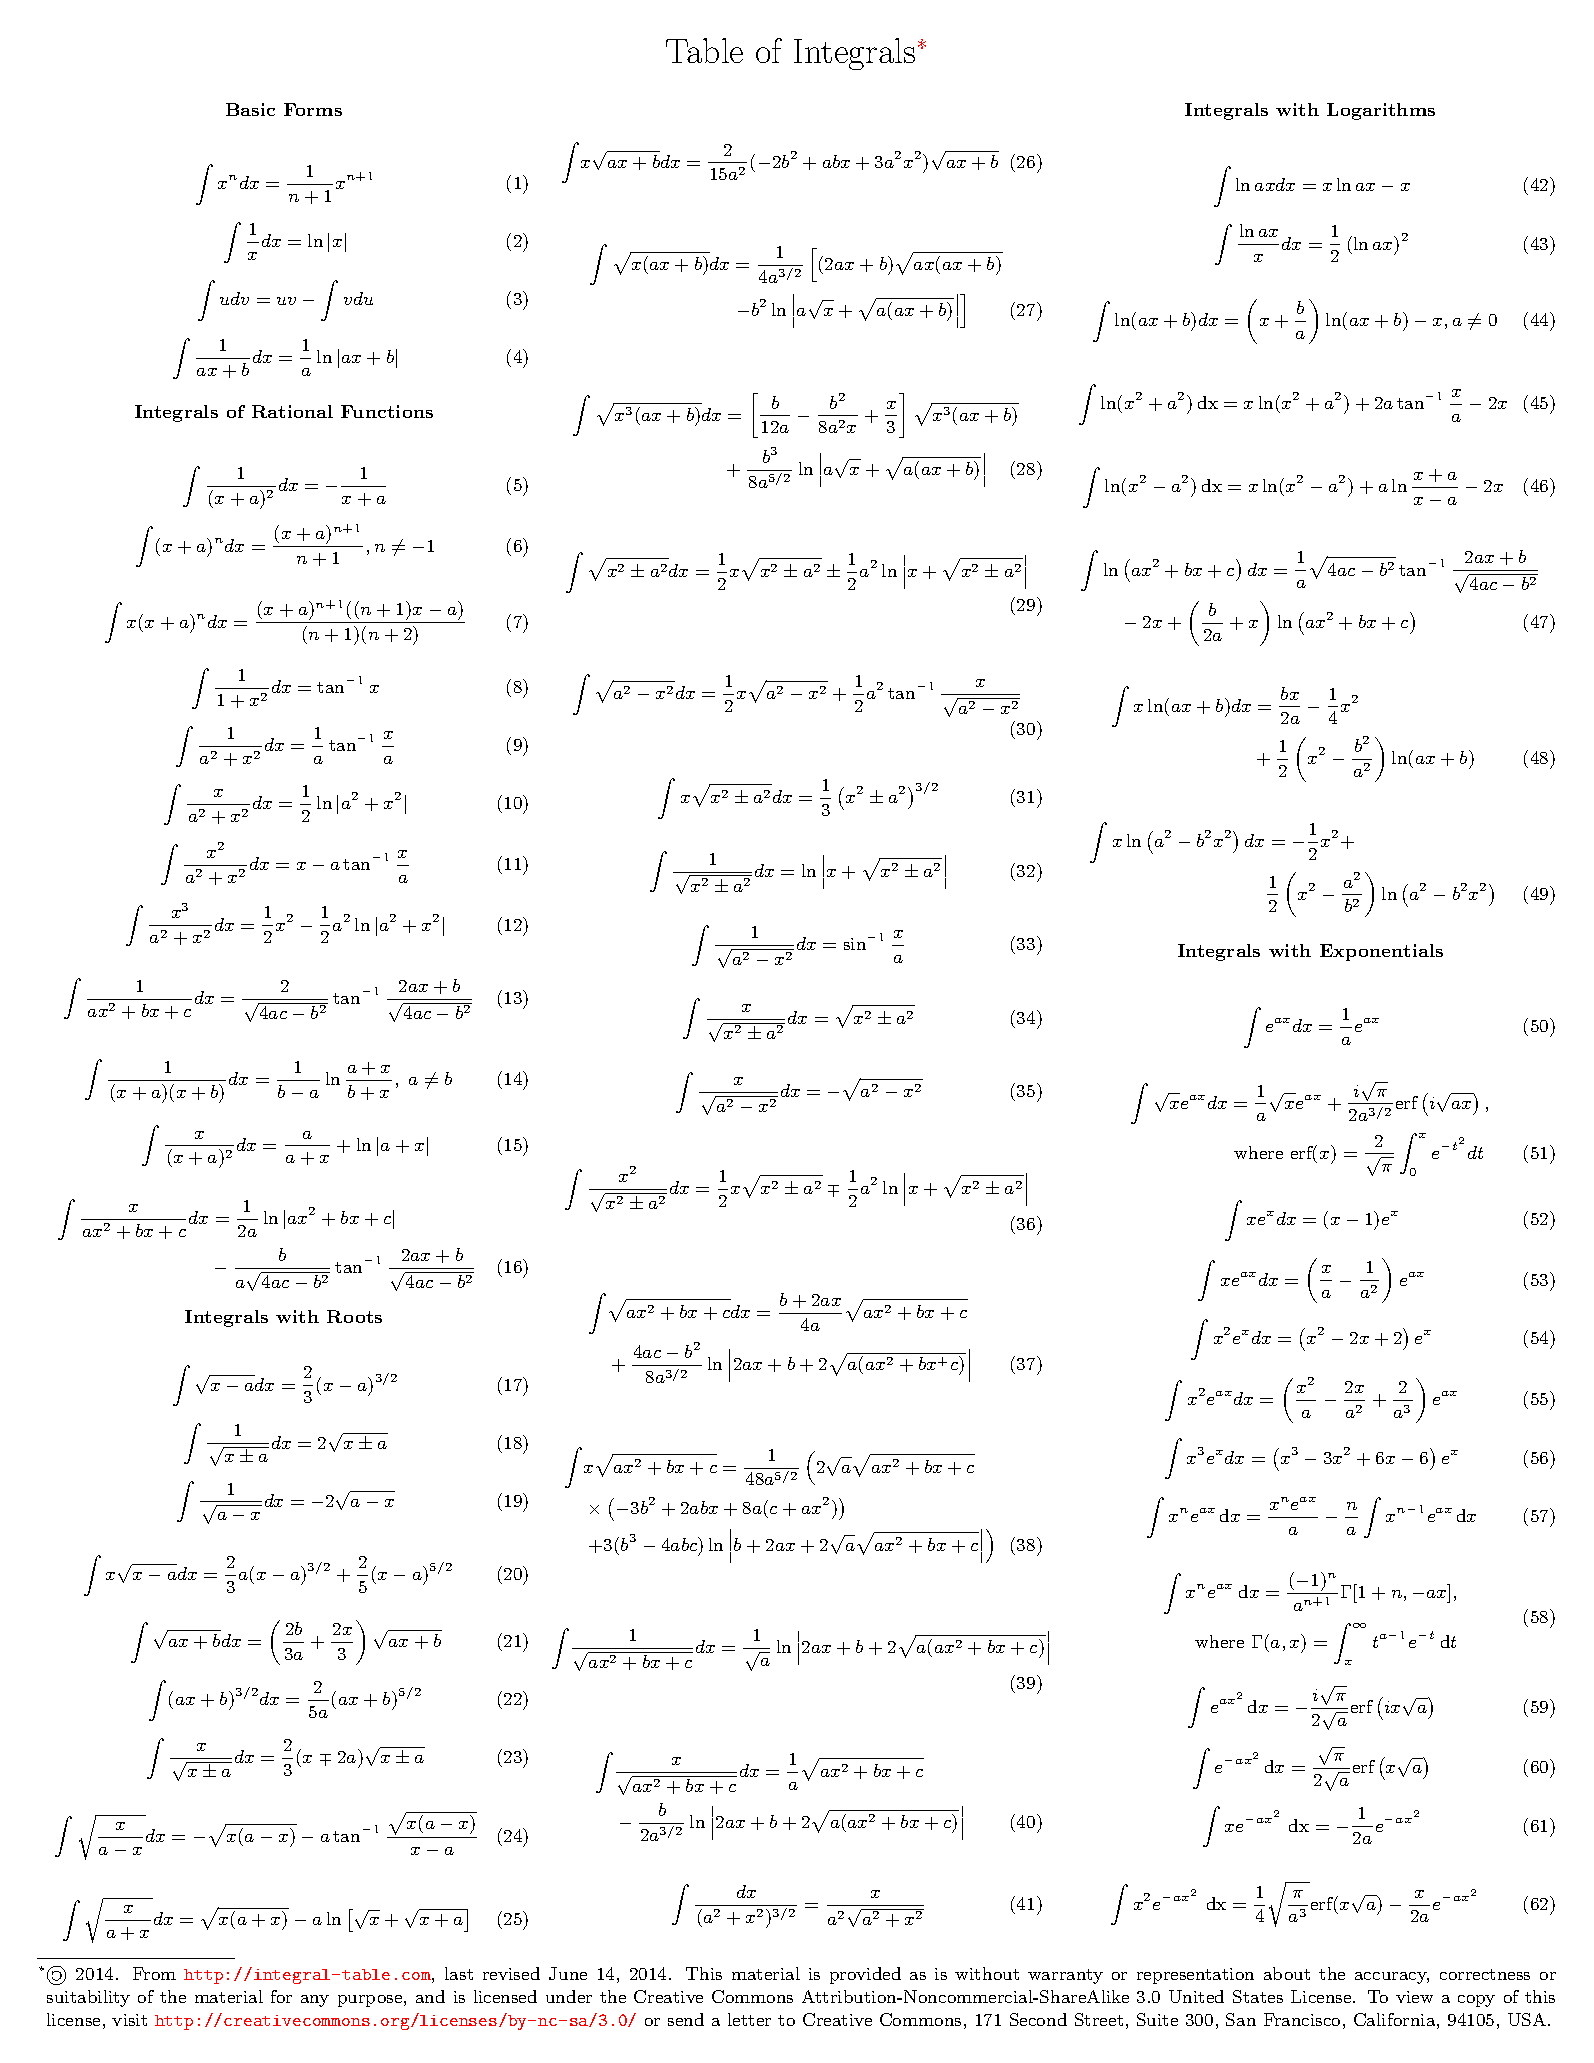
\includepdf[pages=-,pagecommand={\pagestyle{fancy}}]{final/stuff/integralTable.pdf}

%\newpage
%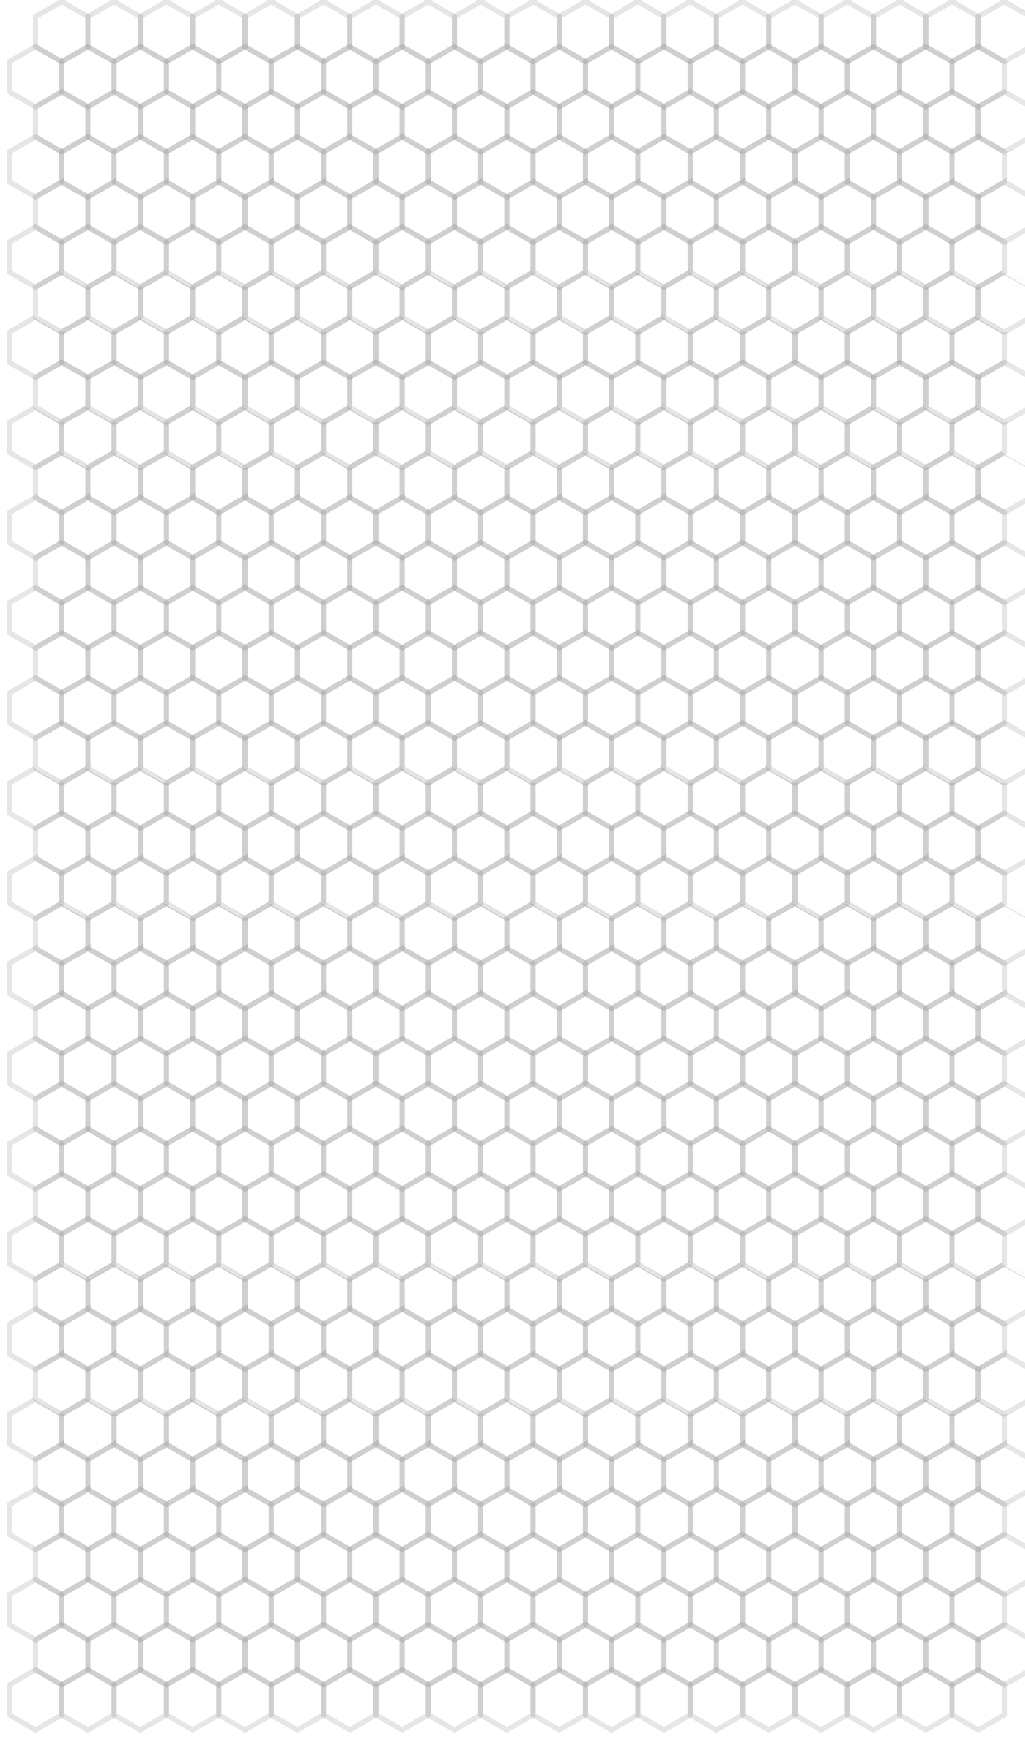
\includepdf[pages=-,pagecommand={\pagestyle{fancy}}]{final/stuff/hexagonal.pdf}
%\newpage
%\twocolumn[
%
\includegraphics{final/stuff/hexagonal.ps}
%]

%\begin{center}
%
\includegraphics{final/stuff/hexagonal.ps}
%\end{center}


%\end{landscape}
\end{document}